% \documentclass[aip,jcp,preprint,unsortedaddress,a4paper,onecolum]{revtex4-1}
\documentclass[aip,jcp,a4paper,reprint,onecolumn]{revtex4-1}
% \documentclass[aps,pre,twocolumn]{revtex4-1}
% \documentclass[aps,jcp,groupedaddress,twocolumn,unsortedaddress]{revtex4}

\usepackage[fleqn]{amsmath}
\usepackage{amssymb}
\usepackage[dvips]{graphicx}
\usepackage{color}
\usepackage{tabularx}
\usepackage{algorithm}
\usepackage{algorithmic}

\makeatletter
\makeatother

\newcommand{\recheck}[1]{{\color{red} #1}}
\newcommand{\redc}[1]{{\color{red} #1}}
\newcommand{\bluec}[1]{{\color{blue} #1}}
\newcommand{\greenc}[1]{{\color{green} #1}}
\newcommand{\vect}[1]{\textbf{\textit{#1}}}
\newcommand{\dd}[0]{\textsf{d}}

\newcommand{\AT}{{\textrm{{AT}}}}
\newcommand{\EX}{{\textrm{EX}}}
\newcommand{\CG}{{\textrm{CG}}}
\newcommand{\HY}{{\Delta}}
\newcommand{\rdf}{{\textrm{rdf}}}
\newcommand{\thf}{{\textrm{th}}}
\newcommand{\dof}{{\textrm{dof}}}
\newcommand{\res}{{\textrm{rep}}}
\newcommand{\ext}{{\textrm{extra}}}
\newcommand{\exc}{{\textrm{exc}}}
\newcommand{\thermo}{{\textrm{Q}}}
\newcommand{\hadress}{{\textrm{H}}}
\newcommand{\dadress}{{\textrm{D}}}
\newcommand{\mh}{\mathcal H}
\newcommand{\kin}{\textrm{kin}}
\newcommand{\trans}{\textrm{T}}
\newcommand{\footh}{\textrm{\tiny H}}
\newcommand{\footo}{\textrm{\tiny O}}
\newcommand{\dgenq}{\dot{\underline{\vect q}}}
\newcommand{\dgenp}{\dot{\underline{\vect p}}}
\newcommand{\genq}{{\underline{\vect q}}}
\newcommand{\genp}{{\underline{\vect p}}}


\begin{document}

\subsection{The eigen modes of the velocity}

We use the following formula to calculate the $k$ mode of the velocity profile:
\begin{align}
  A_k =\bigg\langle \frac 1N \sum_{i=0}^{N-1} v_{i, x} \sin[k\, (r_{i,z} - \frac12 L_z)]\bigg\rangle
\end{align}
Here $N$ is the number of molecules in the system, $v_{i, x}$ is the
$x$ compnent of the velocity of the $i$-th molecule, $r_{i,z}$ is the
$z$ component of the position of the $i$-th molecule. $L_z$ is
simulation box size on the $z$ direction (it is larger than
$2h$). Since the box starts at $(0,0,0)$, the $\sin$ function is
shifted by half of the box size. $\langle\cdot\rangle$ denotes the
ensemble average, by the ergodicity of the system, it can be estimated
by the time average of the corresponding instantenous quantity.

We want to check the equipartition property of the system:
\begin{align}
  2S \int_0^h A_k^2 \sin^2 (k\, z) \,dz = \rho_0k_BT
\end{align}
The integral can be analytically calculated by:
\begin{align}
  \int_0^h\sin^2 (k\, z) \,dz  = \frac{2kh - \sin(2kh)}{4k}
\end{align}
In practice, the integral bound $h$ is determined by substracting the minimum $z$ coordinate
from the maximum $z$ coordinate of the liquid molecules, and then divided by 2:
\begin{align}
  h = \frac12 (\max_{i} r_{i,z} - \min_i r_{i,z})
\end{align}
It is only calculated from the initial configuration, it can be
checked that the value of $h$ does not varies a lot with respect to
time.  Therefore, we should check:
\begin{align}\label{eq:tmp3}
  \frac{2kh - \sin(2kh)}{2k} A_k^2 S = \rho_0 k_BT
\end{align}
In Fig.~\ref{fig:tmp1}, we plot the RHS of Eq~\ref{eq:tmp3} as a function of mode $k$
for different systems.
\begin{figure}
  \centering
  \includegraphics[]{fig/fig-energy.eps}
  \caption{The RHS of Eq~\ref{eq:tmp3} as a function of mode $k$}
  \label{fig:tmp1}
\end{figure}

In Fig.~\ref{fig:tmp3} we show the result of several realizations of system 26.
\begin{figure}
  \centering
  \includegraphics[]{fig/fig-compare.eps}
  \caption{Several realizations of the system 26.}
  \label{fig:tmp3}
\end{figure}

\subsection{The eigen modes of the squared velocity}

Similarly we can calculate the modes of the squared velocity by the
following formulus:
\begin{align}
  B_k =\bigg\langle \frac 1N \sum_{i=0}^{N-1} v^2_{i} \sin[k\, (r_{i,z} - \frac12 L_z)]\bigg\rangle
\end{align}
For simplicity, in Fig.~\ref{fig:tmp2} we plot only the value of $B_k$.
\begin{figure}
  \centering
  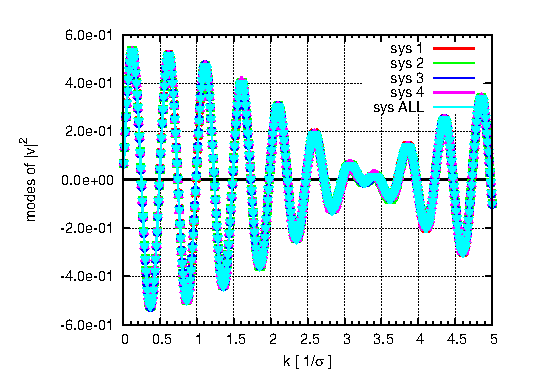
\includegraphics[]{fig/fig-compare-mode2.eps}
  \caption{The modes $B_k$ of the squared velocity.}
  \label{fig:tmp2}
\end{figure}



\end{document}





